

\documentclass{scrartcl}

\usepackage{hyperref}
\usepackage{fontspec}
\usepackage{csquotes}
\usepackage{abstract}
\usepackage{lstlisting}

% Main font
\setmainfont{Baskerville}

% Section numbers
\usepackage{titlesec}
\titleformat*{\section}{\Large\centering}

% Margins
\usepackage[top=3cm, left=4cm, right=4cm, bottom=3cm]{geometry}

\usepackage{titling}

\usepackage{scrpage2}
\pagestyle{scrheadings}
\ohead{McClure}

% Image scaling
\usepackage{graphicx,grffile}
\makeatletter
\def\maxwidth{\ifdim\Gin@nat@width>\linewidth\linewidth\else\Gin@nat@width\fi}
\def\maxheight{\ifdim\Gin@nat@height>\textheight\textheight\else\Gin@nat@height\fi}
\makeatother
\setkeys{Gin}{width=\maxwidth,height=7cm,keepaspectratio}

% Paragraph indents
\setlength{\parskip}{6pt plus 2pt minus 1pt}
\setlength{\parindent}{0pt}

% Footnotes
\usepackage[hang,flushmargin]{footmisc}
\interfootnotelinepenalty=10000
\setlength{\footnotesep}{0.5cm}

% Curly quotes
\newif\ifquoteopen
\catcode`\"=\active
\DeclareRobustCommand*{"}{%
   \ifquoteopen
     \quoteopenfalse ''%
   \else
     \quoteopentrue ``%
   \fi
}


\begin{document}

\title{%
  \vspace{-2cm}Headlines as networked language\vspace{1ex} \\
  \large A study of content and audience across 73 million links on Twitter
}

\author{David McClure}

\date{January 15, 2019}

\maketitle

\section{Introduction}


Imagine that someone showed you a headline from a news article, but in complete isolation, stripped of all context -- just a sequence of words. All they told you is that the headline came from either the New York Times or Fox, and asked you to guess which one. In some cases, this might be fairly easy. For example, if it's a recipe -- we might remember that The New York Times has a large cooking section:

\begin{itemize}
\item Chicken Thighs With Cumin, Cayenne and Citrus
\end{itemize}

Or, if it's about (both) New York baseball teams:

\begin{itemize}
\item In Early Going, the Yankees Steal the Mets' Thunder
\end{itemize}

(Though, of course, Fox also does plenty of sports reporting.) Meanwhile, we might associate a story about MS13 with Fox, to the extent that right-leaning outlets have focused more attention on immigration and crime:

\begin{itemize}
\item East Coast MS 13 gang leader admits racketeering conspiracy
\end{itemize}

But, other things might be significantly harder. For example -- one of these headlines came from Fox, the other from The New York Times:

\begin{itemize}
\item Zambia's 1st female fighter pilot says she "doesn't feel like a woman" in her job
\item 4 freed from Thailand cave, but rescuers face "war with water and time" to get to others
\end{itemize}

Here, to my eye, there aren't obvious "tells" -- there are small things that might push me in one direction or the other, but it's not clear. (The answer -- NYT, Fox.) In trying to guess the outlet, we'd have to bring to bear a wide set of intuitions about what might be thought of as the "voice" of the outlet -- the set of issues, locations, people that the outlet tends to focus on. And, beyond the raw content of what's being -- \textit{how} it's being covered, the style, intonation, attitude, affect. Trying to guess the outlet, in other words, would force us to formalize a kind of mental model about precisely how the two outlets are similar or different.

It also, indirectly, gives a way to reason about the \textit{degree} to which they're similar or different. Now, imagine that instead of just doing this once, we did it for 100 headlines, and counted up the number of correct guesses. We'd likely do better than random -- but how much better? 60\%, 70\%, 95\%? How differentiable are NYT and Fox? To put this into context -- what if we then swapped out the outlets -- pulled headlines from NYT and CNN, instead of NYT and Fox, for example -- and repeated the experiment. We might guess that NYT and CNN are more similar, harder to tell apart. But, how true is this, exactly? Say we got 80 headlines right for the NYT vs. Fox comparison -- would we get 70, 60, 55 right for NYT vs. CNN? In a rough sense, we could start to reason about the relative proximities between different pairs of outlets.

Of course, doing this manually, it would be hard to scale beyond a few outlets and a couple hundred headlines. But -- what if we could do this at a much larger scale, across dozens of different media organizations and millions of headlines? This thesis explores this question as a \textit{language engineering task}, working with a corpus of 73,198,274 tweets harvested from the Decahose over an 18 month period, each containing a link to an article from one of 15 major news organizations. To what degree is it possible to train machine learning models to differentiate between headlines produced by different news outlets? Unlike other studies that have explored the tractability of language inference tasks on news data, though, goal here isn't to solve a literal engineering task (flagging "clickbait" headlines, optimizing click-through rates) -- instead, we use the predictive models as a descriptive and interpretive tool. By training models to differentiate between content from different sources, we can then crack open the hood and examine the representations that are induced by the models; which then makes it possible to "map" headlines as a kind of conceptual space.

Most fundamentally, beyond this ability to "read" headlines at a scale that would otherwise be impossible -- these models make it possible to start filling in a kind of ground-truthed understanding of the degree to which different outlets are similar and different, where we might otherwise have to rely on intuition and anecdote. Modeling a complete matrix of pairwise similarities across 15 major media organizations, we can construct a kind of "content graph," a fully-connected representation how, and to what degree, outlets produce (dis)similar headlines:

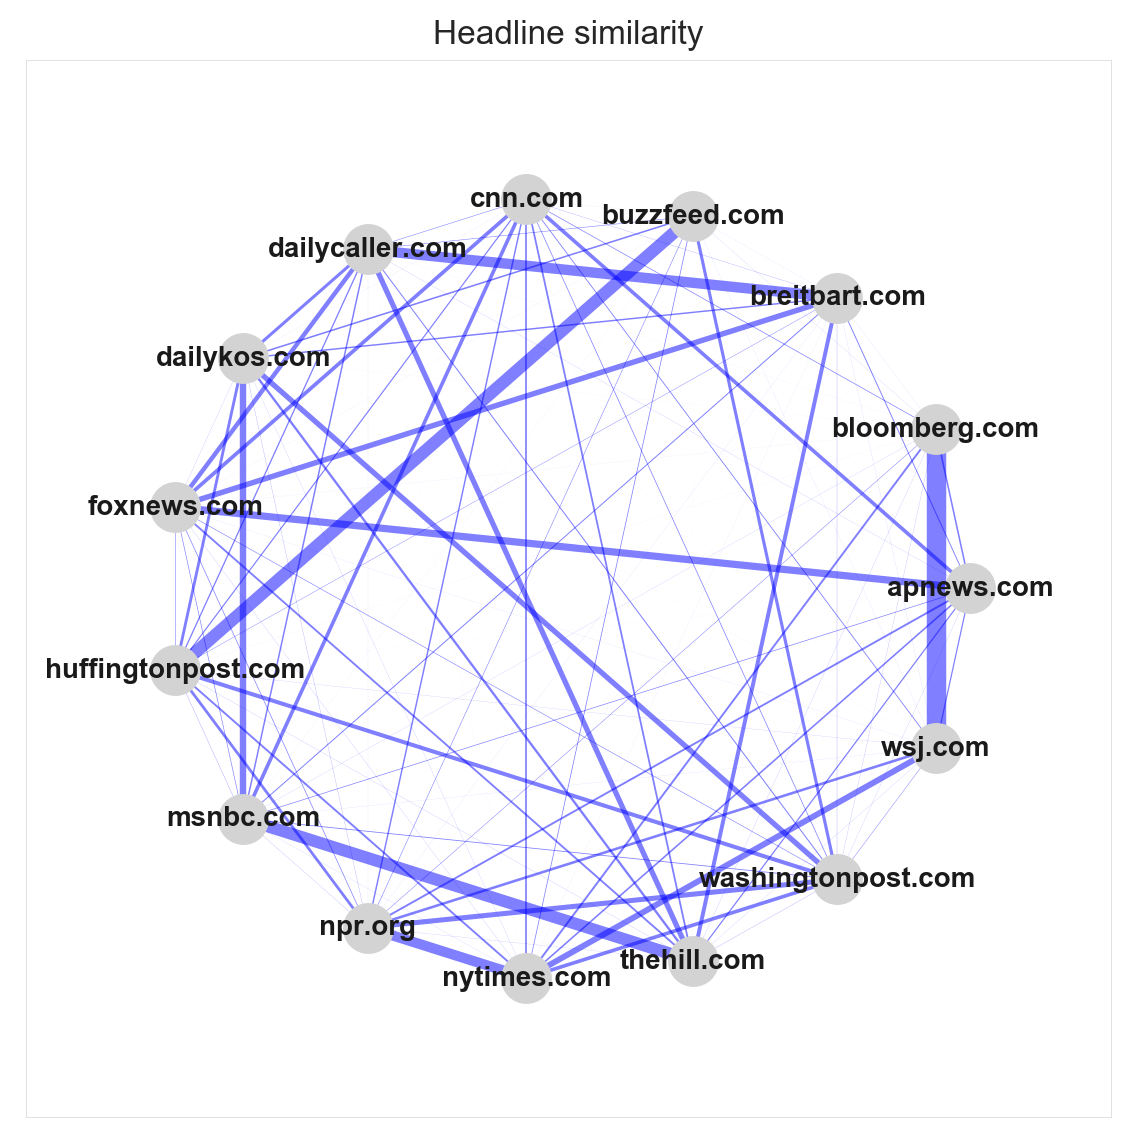
\includegraphics[width=10cm]{figures/hl-graph.png}

Once we have this empirical view of the linguistic proximities among the outlets, though, there's a way in which this immediately just generates a new set of questions. Most of which, really, are some version of just one -- where is this graph not what we would expect? To return to the analogy of voice -- are there outlets that are "speaking" in ways that don't map onto assumptions about the role that they play in a broader political, commercial, historical context?

The second half of the thesis takes up this question, and explores the degree to which these linguistic relationships correspond (and don't correspond) to two different backdrops. First -- we explore the degree to which these similarities at the level of content align with similarities at the level of audience. parallel to the "content graph" defined by the headline similarities, can imagine an "audience graph" that represents similarities at the level of the people who read and distribute content from each pair of outlets.

This question of the interaction between content and audience cuts to the core of a wide range of recent discussions about processes of fragmentation and polarization in the news ecosystem. For example, the widely popularized notions of "filter bubbles" and "echo chambers," where the concern is that these two graphs are tightly connected in a self-reinforcing (and socially problematic) way -- media sources that are highly differentiated at the level of content allow people with different perspectives to self-select into highly differentiated information ecosystems, which, in a vicious circle, then aggravates the underlying social and ideological fragmentation. Stark divisions at the level of content get mirrored by stark differences in audience, which in turn incentivize even more differentiated content, etc.

The graph above, though, suggests there might be places where this alignment between content and audience breaks down. For example, it looks like headlines from Fox are about as similar to headlines from AP as from Breitbart; whereas, we might guess that the audience overlap between Fox and Breitbart would be significantly higher. This suggests a rich set of questions -- are there outlets that "sound" similar to one another, but that have highly non-overlapping audiences? Or, zooming back to the complete ecosystem of media organizations, can we identify outlets that act as "mediators" or "bridges" between different subsets of audiences? For example -- are there outlets that produce content that "sounds like" content produced by left-leaning outlets, but that have relatively high audience overlap with right-leaning outlets -- that is, outlets that produce content that has the effect of exposing right-leaning readers to content that's more typical of left-leaning news feeds? Or vice versa?

These incongruities, misalignments, places where the language graph doesn't map easily onto the underlying social graph -- do they exist at all? If so -- what do they look like? What kind of content does this? Looking beyond this study, which is fundamentally descriptive -- if we're interested in exploring the degree to which different topics, styles, idioms, and ways of speaking might have the effect of working against patterns of fragmentation in media consumption habits, these sites of mismatch could be of particular interest. They would represent, in a sense, naturally-occurring short-circuits between otherwise entrenched associations between particular audiences and particular types of content, places where audiences move (or get moved) out of their typical "lanes."

Second -- building on this question of movement or change, we explore the degree to which the matrix of linguistic similarities has evolved over historical time -- the degree to which it does and doesn't correspond to previous versions of itself. Instead of rolling up the entire 18-month window of data into a single, synchronic unit, we analyze the set of 73 million links as a chronological sequence, covering roughly the first two years of the Trump presidency. Are the linguistic similarities between outlets basically stable, or have there been significant changes over this period? Do outlets drift away from each other, towards each other, back and forth? How fixed or flexible are the major organizations in the media landscape, both in terms of the type of content that they produce and the audiences that read it? And, in the same way that we could explore the overall correlation (and lack thereof) between content and audience -- to what extent do changes in content correspond to changes in audience, when spooled out over historical time? If Huffington Post starts producing headlines that sound more like The Hill -- do the audiences also start to converge?

In summary, this thesis finds:

\begin{enumerate}
\item Modeled as a text classification task, headlines from 15 major US media sources highly differentiable, even after an aggressive cleaning process that strips out any kind of "paratext" in the headline that directly or indirectly reveals the source. (For example, "... -- CNN Video" or "AP Breaking News: ...") The strongest model is a bidirectional LSTM, which gets to 40\% accuracy in a 15-label model (where random would be 7\%). Though, standard non-neural baselines also perform well -- SVM and logistic regression models over ngram count features are competitive at 35-36\% accuracy (and beat the weaker neural models), suggesting that a majority of the differentiability among outlets comes from which words and phrases are being used -- roughly, what might be thought of as "topic" or "content" -- and less from the composition or sequencing of words, which can be modeled with more power by the recurrent models.

\item Pulling sentence embeddings out of the top layer of the LSTM, we can explore the structure of the linguistic space in terms of the high-dimensional representations learned by the model, both in terms of the relationships among different outlets are the internal structure of the headlines within the outlets themselves. This reveals significant differences in what might be thought of as the "shape" of different outlets in the high-dimensional space. Specifically, we focus on what we call the "diameter" of the embedding family for each outlet -- the average cosine distance between randomly sampled pairs of headlines -- which, we argue, roughly captures the degree to which outlets are narrowly focused (low diameter) or more broad and varied (high diameter). Second, we also explore the clustering structure of headlines within outlets, the degree to which content from an outlet can be cleanly decomposed into a set of categories, verticals, or "desks." On both metrics, we find significant variation, with BuzzFeed, Bloomberg, and Daily Kos registering the lowest "diameters" and smallest cluster counts (most focused), and CNN, The Washington Post, and Fox showing the highest diameters / largest cluster counts (most broad, varied, diverse).

\item Aggregating over the full set of individual articles in each outlet, we can use the classifiers to model a complete "content graph" among the 15 organizations, a fully-connected graph of pairwise similarity scores, which are extracted from the behavior of the classifiers in a collection of different ways -- pairwise accuracy scores, probability mass correlations in multi-label models, and confusion counts. With this content graph in hand, we then compare to the underlying "audience graph," derived from correlations in the users who tweet links from each pair of outlets. From these two graphs, for each outlet we can construct two normalized rankings of similarity with all other outlets, one based on headline similarity, and the other based on audience similarity. We then explore the correlation of these two rankings on a per-outlet level -- that is, the degree to which an outlets edge weights in the "content graph" are similar to its edge weights in the "audience graph." In general, we find that these two sets of weights tend to be positively correlated, often highly so -- in general, outlet A "sounds like" outlet B, it also has a high level of audience overlap. But, there is a wide range in the strength of this correlation, and there are two very strong exceptions -- The Hill and AP both have *negatively* correlated weights in the content / audience graphs. Though the specifics are different, in both cases this is broadly because AP and The Hill produce content that resembles, at a linguistic level, content produced by right-leaning outlets; but, the audiences overlap strongly with left-leaning outlets, suggesting that AP and The Hill act as what might be thought of as "one-way bridges" that expose left-leaning audiences to regions of the headline space that are typically focused on by right-leaning outlets. There do no appear to be outlets that perform this function in the opposite direction.

\item We then explore the evolution of these relationships over historical time -- instead of treating the corpora as monolithic bundles of data, the 2-year data window is broken into 100 temporal bins, and a 10-bin rolling window is moved across this space, producing 91 10-bin windows. In each of these windows, we train fully independent A-versus-B models on each unique pair of outlets, and then track changes in these accuracies over time. This reveals significant changes in the structure of the "content graph" in the last two years. First, a cohort of politically-focused outlets have become significantly more similar -- Huffington Post, The Hill, The Daily Kos, and CNN -- suggesting a tendency towards convergence in political coverage since a high-water mark of differentiability in the spring of 2017, in the first months of the Trump administration. Huffington Post in particular has shown the most dramatic shift, moving strongly in the direction of political reporting at the expense of a BuzzFeed-style "listicle" genre that was commonly produced in 2017. Second -- Fox has very consistently moved *away* from almost all other outlets, including other right-leaning outlets like Breitbart and The Daily Caller; it has become much more highly differentiated *individually*, compared to everything else. By examining headlines that typify the overall movement of Fox in the high-dimensional linguistic space modeled by the neural classifier, it appears that this shift is driven by a move in the direction of a highly sensationalized, tabloid style of headline, many of which involve murder or other violent crime.

\item Finally, we also unroll the audience graph over these temporal windows, and explore the degree to which changes in the content graph correlate with changes in the audience graph -- as two outlets produce increasingly similar content, do their audiences also become more overlapping? Overall, we find a positive correlation here, though the relationships for individual pairs of outlets are interestingly varied. In some cases, the content / audience similarities for a pair of outlets move in almost perfect lockstep, sometimes even at the scale of months or weeks -- for example, AP / Huffington Post, Huffington Post / MSNBC, Bloomberg / Fox. But, in other cases, content and audience appear to have an almost perfectly *negative* correlation. For instance, over the last two years, Breitbart and Fox have become very consistently less similar in terms of content, but consistently *more* similar in terms of audience. Or, Breitbart and CNN have had a fluctuating level of similarity at the level of content, and an almost perfectly inverse fluctuation of audience similarity -- when content is similar, audience is dissimilar, and vice versa. These differences suggest that the underlying causal relationships between changes in content and changes in audience are complex, and likely different for different combinations of media organizations.
\end{enumerate}

\section{Headlines on Twitter}

To explore this interaction between content and audience, we need what might be thought of as a "networked" corpus -- a collection of individual pieces of content that can be linked directly to specific patterns of engagement and distribution. With this goal in mind, this study built around a very particular data set -- posts on Twitter that contain links to news articles, which we extract from the Decahose, a 10\% sample of all activity on Twitter. For example, if someone posts a tweet with a link to a New York Times article, Twitter identifies the link and provides structured information about it in the JSON payload that appears in the Decahose:

\begin{lstlisting}[language=Python]
import numpy as np

def incmatrix(genl1,genl2):
    m = len(genl1)
    n = len(genl2)
    M = None #to become the incidence matrix
    VT = np.zeros((n*m,1), int)  #dummy variable

    #compute the bitwise xor matrix
    M1 = bitxormatrix(genl1)
    M2 = np.triu(bitxormatrix(genl2),1)

    for i in range(m-1):
        for j in range(i+1, m):
            [r,c] = np.where(M2 == M1[i,j])
            for k in range(len(r)):
                VT[(i)*n + r[k]] = 1;
                VT[(i)*n + c[k]] = 1;
                VT[(j)*n + r[k]] = 1;
                VT[(j)*n + c[k]] = 1;

                if M is None:
                    M = np.copy(VT)
                else:
                    M = np.concatenate((M, VT), 1)

                VT = np.zeros((n*m,1), int)

    return M
\end{lstlisting}

\end{document}
